\section{Đạo đức, Công bằng \& Quyền riêng tư trong Kỷ nguyên Thị giác AI}
\label{sec:ethics_fairness_privacy}

\subsection{Giới thiệu: Quyền năng đi kèm Trách nhiệm}
\label{subsec:ethics_intro}

Khi Thị giác Máy tính vượt ra khỏi phòng thí nghiệm và trở thành một phần không thể thiếu trong kết cấu xã hội—từ việc quyết định ai được vay vốn, chẩn đoán bệnh tật, cho đến việc xác định một nghi phạm—những câu hỏi về kỹ thuật thuần túy bắt đầu nhường chỗ cho những trăn trở sâu sắc về đạo đức và tác động xã hội. Việc ban cho máy móc khả năng "nhìn" và "phán xét" không chỉ là một thành tựu công nghệ; đó còn là một hành động trao quyền, và quyền năng luôn đi kèm với trách nhiệm.

Một thuật toán có thể đạt độ chính xác 99\% trên một bộ dữ liệu chuẩn hóa, nhưng 1\% sai sót còn lại có thể tập trung một cách có hệ thống vào một nhóm dân tộc thiểu số, dẫn đến những hậu quả tai hại. Một hệ thống camera thông minh có thể giúp quản lý giao thông, nhưng cũng có thể trở thành công cụ giám sát toàn diện, xâm phạm quyền riêng tư ở quy mô chưa từng có. Một mô hình học sâu có thể đưa ra chẩn đoán y khoa chính xác hơn con người, nhưng nếu chúng ta không thể hiểu được "tại sao" nó lại đưa ra quyết định đó, liệu chúng ta có thể tin tưởng và chịu trách nhiệm cho nó?

Phần này không phải là một phụ lục triết học, mà là một phần cốt lõi của cuốn sách. Với tư cách là những nhà khoa học, kỹ sư và người thực hành, chúng ta không chỉ có trách nhiệm xây dựng các hệ thống hoạt động hiệu quả, mà còn phải xây dựng các hệ thống hoạt động một cách \textit{có trách nhiệm}. Chúng ta sẽ đi sâu vào ba trụ cột chính của đạo đức AI trong Thị giác Máy tính:
\begin{itemize}
    \item \textbf{Thiên kiến (Bias) và Công bằng (Fairness):} Khám phá cách các hệ thống AI có thể học và khuếch đại những bất bình đẳng sẵn có trong xã hội, và các phương pháp để giảm thiểu chúng.
    \item \textbf{Quyền riêng tư (Privacy):} Phân tích các rủi ro về việc thu thập và lạm dụng dữ liệu thị giác cá nhân, và các kỹ thuật công nghệ để bảo vệ nó.
    \item \textbf{Trách nhiệm giải trình (Accountability) và Minh bạch (Transparency):} Đối mặt với vấn đề "hộp đen" của các mô hình phức tạp và tìm cách làm cho các quyết định của AI trở nên dễ hiểu và có thể kiểm chứng.
\end{itemize}

Việc trang bị kiến thức về những vấn đề này không phải là một lựa chọn, mà là một yêu cầu bắt buộc đối với bất kỳ ai muốn xây dựng các hệ thống AI có tác động tích cực và bền vững đến thế giới.

\subsection{Thiên kiến (Bias) và Công bằng (Fairness): Khi Dữ liệu Phản ánh Bất bình đẳng}
\label{subsec:bias_and_fairness}

Một trong những lầm tưởng nguy hiểm nhất về AI là nó vốn khách quan vì nó dựa trên toán học và dữ liệu. Thực tế hoàn toàn ngược lại: các mô hình học máy là những tấm gương phản chiếu, và đôi khi là khuếch đại, những thiên kiến tồn tại trong dữ liệu mà chúng được học. Trong Thị giác Máy tính, vấn đề này đặc biệt nghiêm trọng.

\subsubsection{Nguồn gốc của Thiên kiến trong Thị giác Máy tính}
\label{subsubsec:sources_of_bias}
Thiên kiến có thể len lỏi vào một mô hình AI từ nhiều nguồn khác nhau trong vòng đời phát triển của nó.

\begin{description}
    \item[Thiên kiến Dữ liệu (Data Bias):] Đây là nguồn gốc phổ biến và nguy hiểm nhất.
        \begin{itemize}
            \item \textbf{Thiên kiến Lấy mẫu (Sampling Bias):} Dữ liệu được thu thập không đại diện cho phân bố thực tế của thế giới. Ví dụ, các bộ dữ liệu nhận dạng khuôn mặt ban đầu chủ yếu chứa hình ảnh của người da trắng, nam giới \cite{Buolamwini2018}. Kết quả là các mô hình được huấn luyện trên đó có tỷ lệ lỗi cao hơn đáng kể đối với phụ nữ và người da màu.
            \item \textbf{Thiên kiến Đo lường (Measurement Bias):} Cách dữ liệu được thu thập hoặc thiết bị được sử dụng gây ra sai lệch có hệ thống. Ví dụ, các camera rẻ tiền hơn có thể hoạt động kém trong điều kiện ánh sáng yếu, dẫn đến chất lượng ảnh thấp hơn cho các nhóm người dùng có thu nhập thấp, và do đó làm giảm hiệu suất của mô hình đối với nhóm này.
            \item \textbf{Thiên kiến Xã hội (Societal Bias):} Dữ liệu phản ánh các định kiến và bất bình đẳng lịch sử trong xã hội. Ví dụ, một tìm kiếm hình ảnh cho "CEO" có thể trả về phần lớn là hình ảnh nam giới, trong khi "y tá" lại trả về phần lớn là phụ nữ. Một mô hình học từ dữ liệu này có thể củng cố các định kiến nghề nghiệp theo giới tính.
        \end{itemize}
    
    \begin{center}
        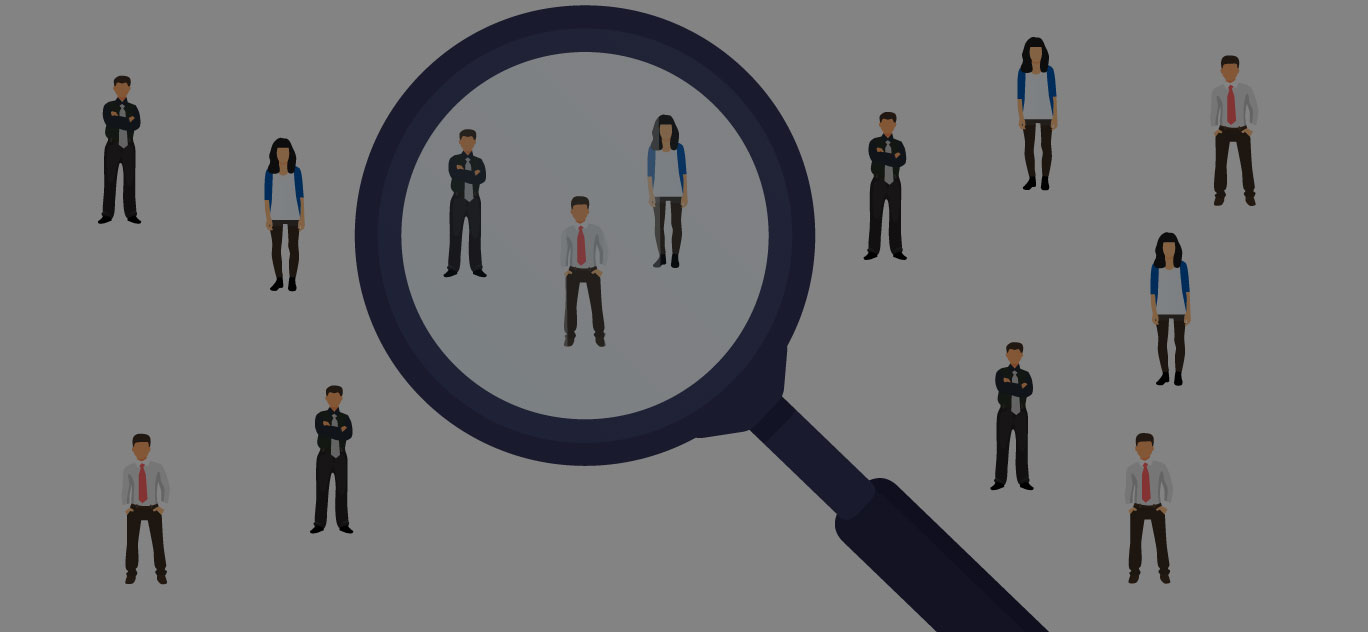
\includegraphics[width=0.9\textwidth]{images/dataset_bias.jpg}
        \captionof{figure}{Minh họa về thiên kiến trong bộ dữ liệu. Một bộ dữ liệu được cho là dùng để nhận dạng "người", nhưng phần lớn hình ảnh lại được thu thập ở một khu vực. Mô hình được huấn luyện trên đó có thể hoạt động kém khi triển khai ở các khu vực địa lý khác, nơi có sự khác biệt về trang phục, bối cảnh và nhân khẩu học.}
        \label{fig:dataset_bias}
    \end{center}
    
    \item[Thiên kiến Thuật toán (Algorithmic Bias):] Bản thân thuật toán, ngay cả khi được huấn luyện trên dữ liệu hoàn hảo, cũng có thể tạo ra hoặc khuếch đại thiên kiến.
        \begin{itemize}
            \item \textbf{Khuếch đại Sai số (Error Amplification):} Nếu một mô hình có tỷ lệ lỗi cao hơn một chút đối với một nhóm thiểu số, các hệ thống vòng lặp kín (ví dụ: một hệ thống đề xuất nội dung) có thể khuếch đại sai sót này theo thời gian, dần dần loại trừ nhóm đó ra khỏi các tương tác tích cực.
            \item \textbf{Hàm mục tiêu không phù hợp (Objective Function Mismatch):} Việc tối ưu hóa cho độ chính xác tổng thể có thể che giấu hiệu suất kém trên các nhóm thiểu số. Một mô hình có độ chính xác 99\% vẫn có thể có tỷ lệ lỗi 50\% trên một nhóm chỉ chiếm 2\% dân số.
        \end{itemize}
        
    \item[Thiên kiến Con người (Human Bias):] Thiên kiến của người gán nhãn hoặc người phát triển.
        \begin{itemize}
            \item \textbf{Thiên kiến Gán nhãn (Label Bias):} Các nhãn được gán cho dữ liệu có thể mang tính chủ quan hoặc định kiến. Ví dụ, người gán nhãn có thể có xu hướng gán nhãn "hung hăng" cho các biểu cảm trên khuôn mặt của một nhóm người nhất định nhiều hơn các nhóm khác.
        \end{itemize}
\end{description}

\subsubsection{Hậu quả trong Thế giới Thực}
\label{subsubsec:real_world_consequences}
Thiên kiến trong các hệ thống CV không phải là vấn đề lý thuyết. Nó gây ra những tác hại thực sự:
\begin{itemize}
    \item \textbf{Hệ thống Tư pháp Hình sự:} Các hệ thống nhận dạng khuôn mặt thiên vị có thể dẫn đến việc nhận dạng sai và bắt giữ oan sai, đặc biệt là đối với các nhóm thiểu số.
    \item \textbf{Tuyển dụng:} Các công cụ AI sàng lọc hồ sơ hoặc phân tích phỏng vấn video có thể bị thiên vị chống lại các ứng viên nữ hoặc các ứng viên có ngoại hình không theo "chuẩn".
    \item \textbf{Y tế:} Một thuật toán chẩn đoán ung thư da được huấn luyện chủ yếu trên hình ảnh của người da trắng có thể bỏ sót các dấu hiệu bệnh trên người da màu, nơi các biểu hiện của bệnh có thể khác biệt.
    \item \textbf{Xe tự lái:} Nếu một hệ thống phát hiện người đi bộ được huấn luyện chủ yếu với dữ liệu ban ngày, nó có thể hoạt động kém hiệu quả vào ban đêm hoặc đối với những người có màu da tối hơn, đặt họ vào tình thế nguy hiểm hơn.
\end{itemize}

\subsubsection{Các phương pháp hướng tới Sự Công bằng (Fairness)}
\label{subsubsec:mitigating_bias}
Giải quyết thiên kiến là một thách thức phức tạp, đòi hỏi sự can thiệp ở nhiều cấp độ.
\begin{enumerate}
    \item \textbf{Tiền xử lý (Pre-processing):} Tập trung vào dữ liệu.
        \begin{itemize}
            \item \textbf{Kiểm tra và Đa dạng hóa Dữ liệu:} Sử dụng các công cụ như "Datasheets for Datasets" \cite{Gebru2021} để ghi lại nguồn gốc, thành phần và các hạn chế của bộ dữ liệu. Tích cực thu thập thêm dữ liệu cho các nhóm đang bị thiếu đại diện.
            \item \textbf{Tăng cường Dữ liệu có ý thức (Fairness-aware Augmentation):} Áp dụng các kỹ thuật tăng cường dữ liệu một cách có chọn lọc để cân bằng lại tập dữ liệu.
        \end{itemize}
    \item \textbf{Xử lý trong quá trình (In-processing):} Sửa đổi thuật toán học tập.
        \begin{itemize}
            \item \textbf{Thêm ràng buộc Công bằng:} Thêm các thành phần vào hàm mất mát để phạt các mô hình đưa ra các dự đoán khác nhau cho các nhóm khác nhau.
            \item \textbf{Học Đối kháng để Giảm Thiên kiến (Adversarial Debiasing):} Huấn luyện đồng thời hai mạng: một mạng chính để thực hiện tác vụ, và một mạng "đối thủ" cố gắng dự đoán thuộc tính nhạy cảm (ví dụ: giới tính, chủng tộc) từ các đặc trưng của mạng chính. Mạng chính được huấn luyện để vừa hoàn thành tốt tác vụ, vừa "đánh lừa" mạng đối thủ, qua đó học được các biểu diễn ít chứa thông tin về thuộc tính nhạy cảm hơn.
        \end{itemize}
    \item \textbf{Hậu xử lý (Post-processing):} Điều chỉnh đầu ra của mô hình.
        \begin{itemize}
            \item \textbf{Hiệu chỉnh Ngưỡng:} Điều chỉnh ngưỡng quyết định (ví dụ: ngưỡng để xác định một khuôn mặt là "khớp") cho các nhóm khác nhau để đảm bảo các tỷ lệ lỗi (ví dụ: dương tính giả) là như nhau.
        \end{itemize}
\end{enumerate}

\subsection{Quyền Riêng tư (Privacy): Bảo vệ Dấu vân tay Kỹ thuật số}
\label{subsec:privacy}

Hình ảnh và video, đặc biệt là những hình ảnh có mặt người, là một trong những dạng dữ liệu cá nhân nhạy cảm nhất. Các hệ thống CV, với khả năng phân tích và nhận dạng ở quy mô lớn, đặt ra những thách thức lớn về quyền riêng tư.

\subsubsection{Các Rủi ro về Quyền Riêng tư}
\label{subsubsec:privacy_risks}
\begin{itemize}
    \item \textbf{Giám sát và Theo dõi (Surveillance and Tracking):} Việc triển khai rộng rãi các hệ thống camera kết hợp với nhận dạng khuôn mặt có thể tạo ra một cơ sở hạ tầng giám sát vĩnh viễn, cho phép theo dõi chuyển động của công dân mà không cần sự đồng ý của họ.
    \item \textbf{Tái nhận dạng (Re-identification):} Ngay cả khi dữ liệu đã được "ẩn danh" (ví dụ: bằng cách làm mờ khuôn mặt), các thuật toán vẫn có thể tái nhận dạng một người dựa trên các đặc điểm khác như dáng đi, quần áo, hoặc bối cảnh.
    \item \textbf{Suy luận Thuộc tính Nhạy cảm (Inference of Sensitive Attributes):} Các mô hình CV có thể được huấn luyện để suy luận các thông tin cực kỳ riêng tư từ hình ảnh, chẳng hạn như tình trạng sức khỏe, cảm xúc, khuynh hướng tình dục, hoặc quan điểm chính trị, chỉ từ một bức ảnh chân dung hoặc một đoạn video ngắn.
    \item \textbf{Tấn công Đảo ngược (Model Inversion Attacks):} Trong một số trường hợp, kẻ tấn công có thể cố gắng tái tạo lại một phần dữ liệu huấn luyện (ví dụ: hình ảnh khuôn mặt của một người) chỉ bằng cách truy vấn mô hình đã được huấn luyện.
\end{itemize}

\subsubsection{Các Kỹ thuật Công nghệ Nâng cao Quyền riêng tư (Privacy-Enhancing Technologies - PETs)}
\label{subsubsec:privacy_enhancing_tech}
Nhiều kỹ thuật đang được phát triển để cho phép khai thác giá trị từ dữ liệu thị giác mà không xâm phạm quyền riêng tư.
\begin{description}
    \item[Học Liên hợp (Federated Learning) \cite{McMahan2017}:] Thay vì thu thập tất cả dữ liệu thô về một máy chủ trung tâm, mô hình được gửi đến các thiết bị của người dùng (ví dụ: điện thoại). Mô hình được huấn luyện cục bộ trên dữ liệu của người dùng, và chỉ có các bản cập nhật trọng số (các gradient đã được tổng hợp) được gửi về máy chủ để cải thiện mô hình chung. Dữ liệu ảnh và video nhạy cảm không bao giờ rời khỏi thiết bị của người dùng.
    \item[Quyền riêng tư Vi phân (Differential Privacy) \cite{Dwork2006}:] Cung cấp một định nghĩa toán học chặt chẽ về quyền riêng tư. Một thuật toán được cho là có tính riêng tư vi phân nếu việc thêm hoặc xóa dữ liệu của một cá nhân bất kỳ khỏi tập dữ liệu không làm thay đổi đáng kể đầu ra của thuật toán. Điều này thường đạt được bằng cách thêm một lượng nhiễu ngẫu nhiên được kiểm soát cẩn thận vào dữ liệu, các tham số trung gian, hoặc kết quả cuối cùng.
    \item[Mã hóa Đồng cấu (Homomorphic Encryption):] Một dạng mã hóa cho phép thực hiện các phép tính toán trực tiếp trên dữ liệu đã được mã hóa mà không cần giải mã nó trước. Về lý thuyết, điều này cho phép một dịch vụ đám mây huấn luyện một mô hình Thị giác Máy tính trên dữ liệu ảnh đã được mã hóa hoàn toàn, đảm bảo quyền riêng tư tuyệt đối. Tuy nhiên, kỹ thuật này hiện vẫn còn rất tốn kém về mặt tính toán và chưa thực tế cho các mô hình học sâu phức tạp.
\end{description}

\subsection{Trách nhiệm giải trình (Accountability) và Minh bạch (Transparency)}
\label{subsec:accountability_transparency}
Khi một hệ thống AI đưa ra một quyết định quan trọng, ai sẽ chịu trách nhiệm? Và làm thế nào chúng ta có thể tin tưởng một quyết định nếu không hiểu được lý do đằng sau nó?

\subsubsection{Vấn đề "Hộp đen" và Nhu cầu Giải thích được (XAI)}
\label{subsubsec:black_box_xai}
Các mô hình học sâu hiện đại, với hàng tỷ tham số được tối ưu hóa tự động, thường hoạt động như những "hộp đen" (black boxes). Chúng ta biết đầu vào và đầu ra, nhưng quá trình ra quyết định bên trong lại cực kỳ phức tạp và khó diễn giải bằng ngôn ngữ con người. Sự thiếu minh bạch này là một rào cản lớn đối với việc áp dụng AI trong các lĩnh vực có rủi ro cao.

\textbf{AI Giải thích được (Explainable AI - XAI)} là một lĩnh vực nghiên cứu nhằm phát triển các phương pháp giúp con người hiểu và diễn giải các dự đoán của mô hình AI. Trong Thị giác Máy tính, các kỹ thuật XAI phổ biến bao gồm:
\begin{itemize}
    \item \textbf{Bản đồ Saliency (Saliency Maps):} Các kỹ thuật này tạo ra một bản đồ nhiệt (heatmap) phủ lên ảnh đầu vào, làm nổi bật các pixel hoặc vùng ảnh có ảnh hưởng lớn nhất đến quyết định cuối cùng của mô hình. Chúng trả lời câu hỏi: "Mô hình đang nhìn vào đâu?".
    \item \textbf{Grad-CAM (Gradient-weighted Class Activation Mapping) \cite{Selvaraju2017}:} Là một kỹ thuật tạo bản đồ saliency rất phổ biến. Nó sử dụng gradient của lớp dự đoán cuối cùng chảy ngược về lớp tích chập cuối cùng để tạo ra một bản đồ thô, có độ phân giải thấp, cho thấy các vùng quan trọng. Bản đồ này sau đó được nội suy lên kích thước ảnh gốc.
\end{itemize}

\begin{center}
    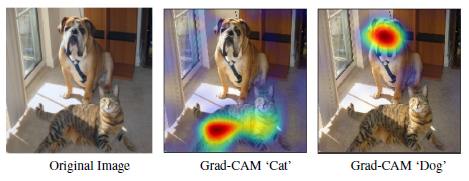
\includegraphics[width=0.8\textwidth]{images/grad_cam.png}
    \captionof{figure}{Ví dụ về Grad-CAM. Để giải thích tại sao mô hình phân loại ảnh này là "chó", Grad-CAM tạo ra một bản đồ nhiệt cho thấy mô hình đang tập trung chủ yếu vào phần đầu và thân của con chó, một hành vi diễn giải hợp lý.}
    \label{fig:grad_cam}
\end{center}

Mặc dù hữu ích, các kỹ thuật XAI hiện tại vẫn còn hạn chế. Chúng chỉ cung cấp một phần của câu chuyện và đôi khi có thể gây hiểu lầm.

\subsubsection{Quản trị và Vòng đời AI có Trách nhiệm}
\label{subsubsec:governance}
Giải quyết các vấn đề đạo đức không chỉ dừng lại ở thuật toán. Nó đòi hỏi một khuôn khổ quản trị toàn diện trong suốt vòng đời của một dự án AI:
\begin{enumerate}
    \item \textbf{Thiết kế:} Đánh giá tác động đạo đức tiềm tàng ngay từ đầu. Xác định các bên liên quan và các rủi ro có thể xảy ra.
    \item \textbf{Dữ liệu:} Quản lý dữ liệu một cách có trách nhiệm, đảm bảo sự đồng ý, quyền riêng tư, và kiểm tra thiên kiến.
    \item \textbf{Mô hình hóa:} Lựa chọn các mô hình và hàm mục tiêu có tính đến sự công bằng và minh bạch. Ghi lại tài liệu về các quyết định đã đưa ra (ví dụ: Model Cards \cite{Mitchell2019}).
    \item \textbf{Triển khai và Giám sát:} Liên tục theo dõi hiệu suất của mô hình trên thực tế, đặc biệt là trên các nhóm dân số khác nhau. Thiết lập các cơ chế để người dùng có thể khiếu nại và sửa chữa các quyết định sai lầm của AI.
\end{enumerate}

\section*{Tài liệu tham khảo}
\begin{itemize}
    \item[1] O'Neil, C. \textit{Weapons of Math Destruction: How Big Data Increases Inequality and Threatens Democracy}. Crown, 2016. (Một cuốn sách kinh điển về tác động xã hội của thuật toán).
    \item[2] Buolamwini, J.; Gebru, T. Gender Shades: Intersectional Accuracy Disparities in Commercial Gender Classification. In \textit{Conference on Fairness, Accountability and Transparency}, 2018. (Nghiên cứu đột phá vạch trần thiên kiến trong các hệ thống nhận dạng khuôn mặt thương mại).
    \item[3] Gebru, T. et al. Datasheets for Datasets. \textit{Communications of the ACM} \textbf{2021}, \textit{64}(12), 86-92.
    \item[4] Mitchell, M. et al. Model Cards for Model Reporting. In \textit{Conference on Fairness, Accountability, and Transparency}, 2019.
    \item[5] McMahan, B. et al. Communication-Efficient Learning of Deep Networks from Decentralized Data. In \textit{Artificial Intelligence and Statistics (AISTATS)}, 2017. (Bài báo giới thiệu khái niệm Học Liên hợp).
    \item[6] Dwork, C. et al. Calibrating noise to sensitivity in private data analysis. In \textit{Theory of Cryptography Conference}, 2006. (Bài báo nền tảng về Quyền riêng tư Vi phân).
    \item[7] Selvaraju, R. R. et al. Grad-CAM: Visual Explanations from Deep Networks via Gradient-based Localization. In \textit{International Conference on Computer Vision (ICCV)}, 2017.
    \item[8] Liu, J.; Jin, Y. A comprehensive survey of robust deep learning in computer vision. \textit{Journal of Automation and Intelligence} \textbf{2023}, \textit{2}, 175-197. (Cung cấp một góc nhìn tổng quan về các vấn đề robustness, có liên quan đến accountability).
\end{itemize}